\chapter{Analyse}
Abschließend soll nun die Funktionalität des TrackCleaners untersucht und bewertet werden. Dazu wird zunächst die Funktionsweise des Cleaners an einem exemplarischen Fall demonstriert. Im Anschluss daran wird das Laufzeitverhalten und die Qualität des Bereinigens analysiert und bewertet. Des Weiteren wird dokumentiert, wie die optimale Distanz, ab welcher ein Hit aussortiert wird, bestimmt wurde.

\section{Analyse der Funktionalität}
Root bietet die Möglichkeit die simulierten Events zu visualisieren. Dazu kommt das Tool Eve zum Einsatz, welches in der Lage ist eine Root-Datei auszulesen und Tracks, Mote-Carlo-Points und Hits graphisch darzustellen. Abbildung \ref{fig:points} zeigt ein Event mit zwei physikalischen Tracks, welche von zwei verschiedenen Teilchen verursacht wurden. Das erste Teilchen(grün) bewegte sich vom Stoßpunkt aus auf einer vergleichsweise geradlinigen Flugbahn aus dem STT heraus. Das zweite Teilchen(weiß) bewegt sich auf einer Kreisbahn mehrere Male durch den STT und kreuzt dabei auch die Flugbahn des ersten Teilchens. Die magentafarbenen Punkte stellen die Ponte-Carlo-Points dar. An diesen Stellen haben die beiden Teilchen also die Straw-Tubes durchflogen. Betrachtet wird nun die Rekonstruktion des grünen Tracks. 

\begin{figure}
  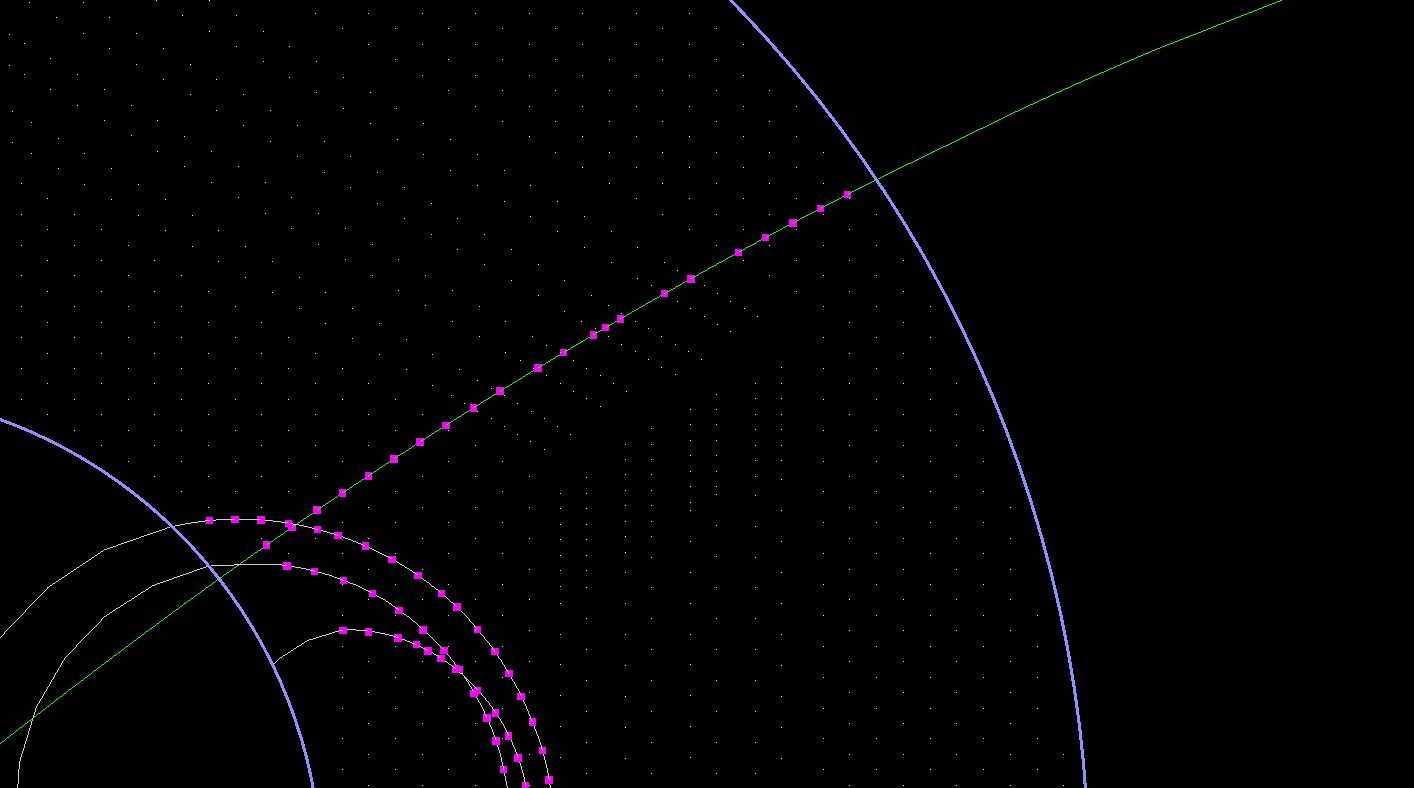
\includegraphics[width=0.9\textwidth]{Bilder/Points2}
	\label{fig:points}
	\caption{Visualisierung eines Events mit zwei Tracks}
\end{figure}

In Abbildung \ref{fig:hits} sind die Hits dargestellt, welche von einem Track-Cleaner diesem Track zugeordnet wurden. In Rot wurde die approximierte Kreisbahn dargestellt. Zunächst fällt auf, dass die Hits im Gegensatz zu den Points nicht direkt auf der Kreisbahn liegen, da sie am Mittelpunkt der getroffenen Straw-Tube dargestellt werden. Folglich besitzen auch die korrekt rekonstruierten Hits meist einen gewissen Abstand vom Track. Außerdem sind die gedrehten Straw-Tubes aus den oben genannten Gründen vom Track entfernt worden. Des Weiteren ist zu bemerken, dass sich am inneren Rand des STTs vier Hits mit einem vergleichsweise großen Abstand zum Track befinden. Beim Vergleich beider Abbildungen lässt sich feststellen, dass sich diesen Punkten keinen Points zuordnen lassen, welche zum grünen Track gehören. In der unmittelbaren Umgebung existieren jedoch einige Points, welche dem weißen Track zuzuordnen sind. Folglich sind diese vier Hits fehlerhaft zugeordnet worden.

\begin{figure}
  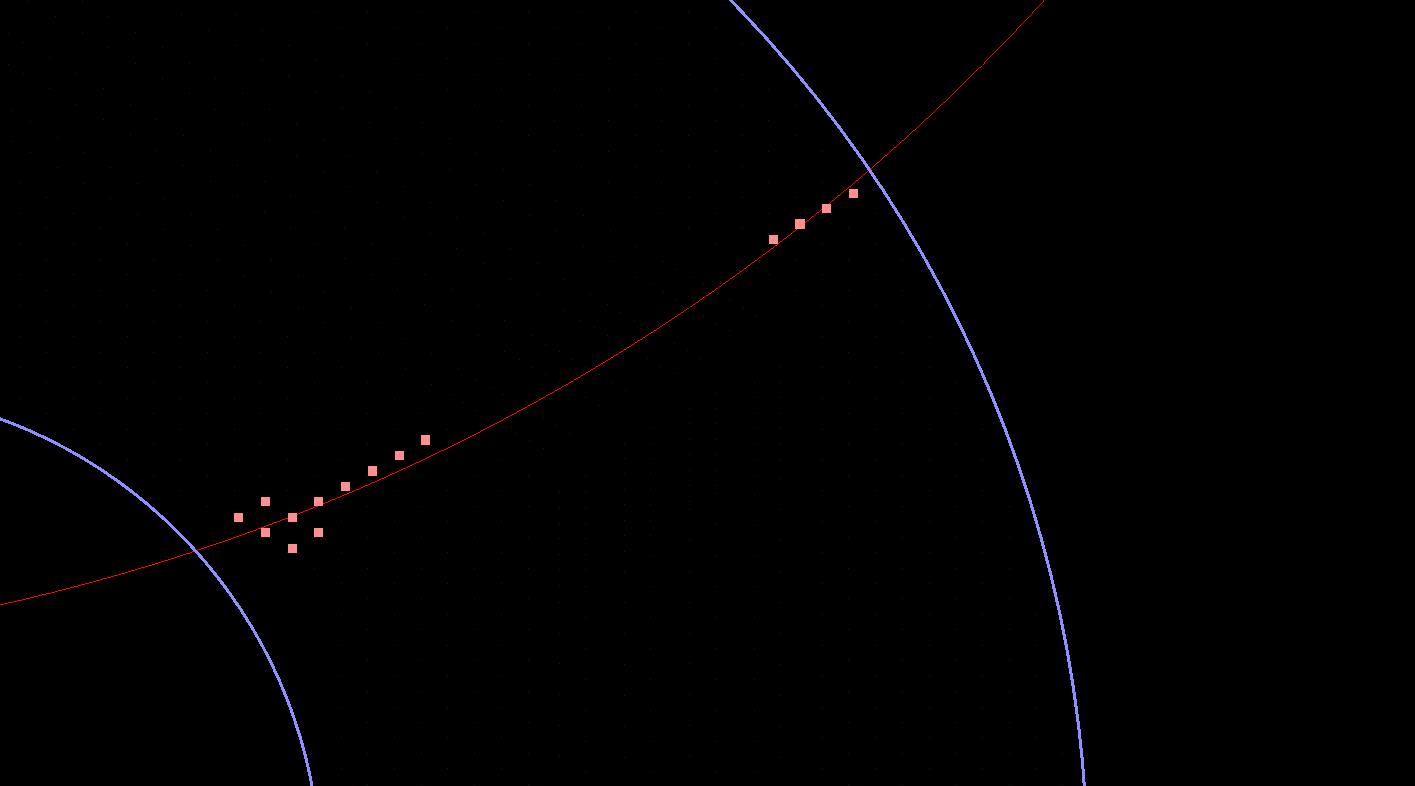
\includegraphics[width=0.9\textwidth]{Bilder/HitsApprox}
	\label{fig:hits}
	\caption{Visualisierung des rekonstruierten Tracks mit den zugeordneten STT-Hits}
\end{figure}

Der vorliegende, rekonstruierte Track wird nun vom TrackCleaner bereinigt. Das Ergebnis ist in Abbildung \ref{fig:cleaned} zu sehen. Es ist zu sehen, dass die beiden unteren fehlerhaften Hits aussortiert worden sind und eine verbesserte Approximation erstellt wurde. Die oberen beiden Fehlerhaften Hits wurden nicht entfernt. Dies hängt damit zusammen, dass im vorliegenden Beispiel die Distanz 0.6 benutzt wurde und die oberen Hits diesen Grenzwert nicht überschreiten.

\begin{figure}
  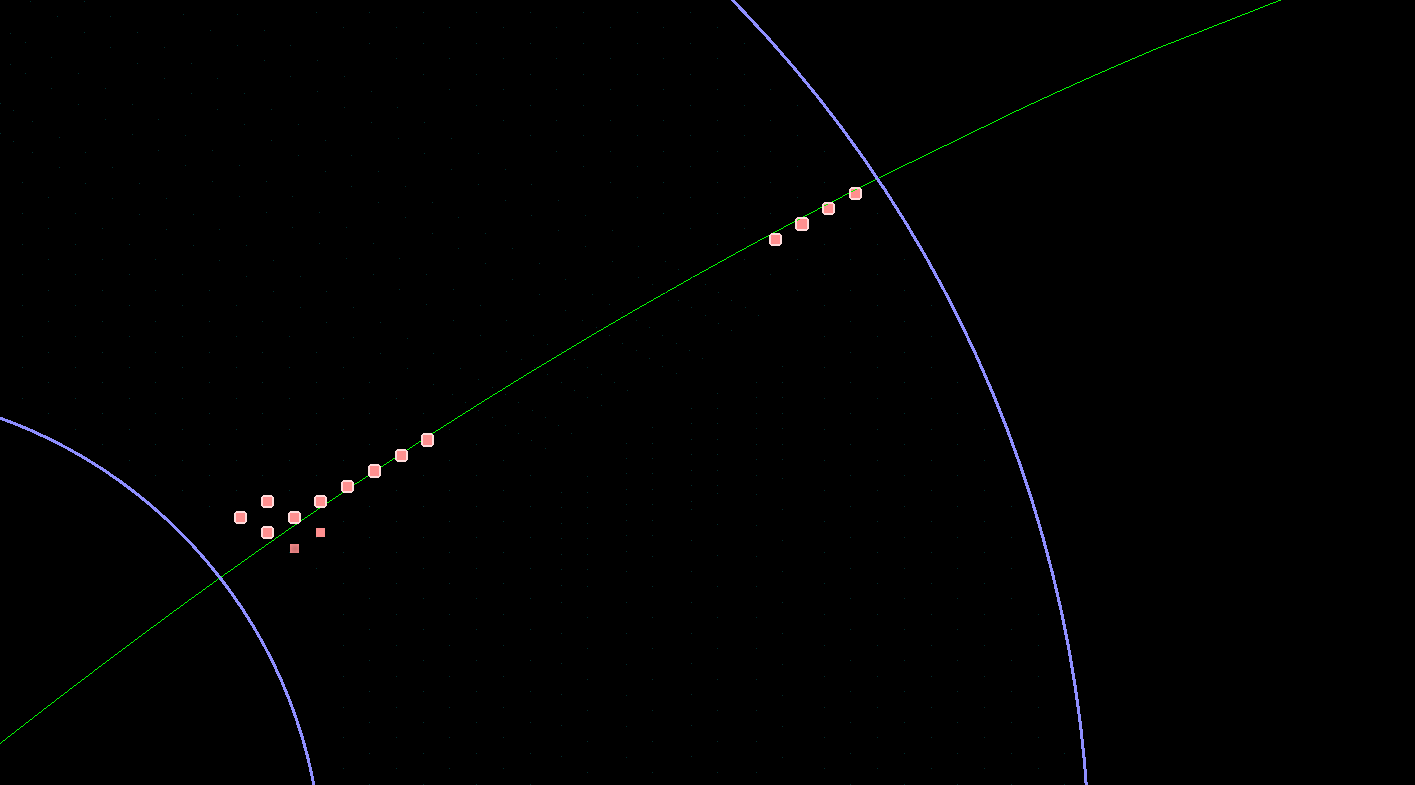
\includegraphics[width=0.9\textwidth]{Bilder/CleanedWithTrack}
	\label{fig:cleaned}
	\caption{Visualisierung des bereinigten Tracks}
\end{figure}

\section{Qualitätsanalyse}
Zur genauen Analyse des Algorithmus wurde eine Analysetask entwickelt. Diese lädt zunächst die Root-Branches CleanedTracks und TracksToClean. Da bei einer Simulation die Daten der physikalischen Tracks vorliegen, ist es nun möglich, zu jedem Hit der beiden Tracks die ID des zugehörigen MC-Tracks zu bestimmen. Im Anschluss daran wird der MC-Track bestimmt, welcher die meisten zugehörigen Hits im zu bereinigten Track enthält. Es wird dann angenommen, dass dieser Track rekonstruiert werden sollte. Alle Hits mit einer identischen Track-ID sind folglich korrekt zugeordnet und alle Hits mit einer anderen Track-ID sind fehlerhaft. Danach werden über die folgende Mengenoperation die Hits bestimmt, welche vom Cleaner aussortiert wurden.

\begin{Definition}
Sei A die Menge der Hits, welche zu einem bereinigten Track gehören und B die Menge der Hits, welche zu dem entsprechenden, noch nicht bereinigten Track gehören. Dann enthält C=B\textbackslash A genau die Hits, welche vom TrackCleaner aussortiert wurden.
\end{Definition}

Abschließend wird dann zu jeden Hit $ h \in C $ die TrackID bestimmt, und somit beurteilt, ob es sich um einen korrekt aussortierten Hit handelt. Das Ergebnis der Analyse wird dann zusammen mit der beim Bereinigen benutzten Distanz an eine CSV-Datei angehängt, um die Ergebnisse später automatisiert weiterverarbeiten zu können.

\section{Laufzeitverhalten}
Bei der Analyse des Laufzeitverhaltens ergaben sich die in \ref{tab: resultsRuntime} dargestellten Ergebnisse. Die Methoden Init und Exec beziehen sich auf die Klasse PndTrackCleanerTask, die Methode Clean bezieht sich auf den PndTrackCleaner.

\begin{figure}
\begin{center}
\begin{tabular}{ |c|c|}
	\hline
	Methode & Laufzeit\\
	\hline
	Init & $6 \cdot 10^{-5} s$ \\
	Exec & $2.027 \cdot 10^{-6} s$\\
	Clean & $7 \cdot 10^{-9} s$\\
	\hline
\end{tabular}
\end{center}
\caption{Ergebnisse der Laufzeitanalyse}
\label{tab: resultsRuntime}
\end{figure}

\section{Bestimmung der optimalen Distanz}
Es soll nun im Rahmen einer Parameterstudie die optimale Distanz bestimmt werden. Dazu wurde ein Skript entwickelt, welches sowohl die Rekonstruktion als auch die Analyse mit unterschiedlichen Distanzen startet. Die CSV Datei wird dann mit den Ergebnissen der Analyse gefüllt. Dabei ergaben sich die in Tabelle \ref{tab: results} dargestellten Ergebnisse. Die hier dargestellte Simulation beinhaltete 1000 Events mit insgesamt 48152 STT-Hits von ausschließlich nicht gedrehten Straw-Tubes. Der erste Eintrag der Tabelle stellt die Ergebnisse dar, welche bei einer Distanz von null erzielt werden. Da hierbei ausnahmslos alle Hits aussortiert werden, macht diese Distanz wenig Sinn, liefert jedoch Informationen über die Beschaffenheit der vorliegenden Stichprobe. Da 1889 Hits korrekt entfernt wurden, hat in diesen Fällen der Trackfinding-Algorithmus einen Fehler gemacht. Die Entfernung der übrigen 46263 Hits war hingegen inkorrekt, folglich wurden diese Hits korrekt zugeordnet.

\begin{figure}
\begin{center}
\begin{tabular}{ |c|c|c|c|}
	\hline
	Distanz & aussortierte Hits & davon korrekt entfernt & davon fehlerhaft entfernt\\
	\hline
0	&   48152 &1889 & 46263\\
0.1	&	12824 & 989	& 11835\\
0.2	&	5144	  & 831	& 4313\\
0.3	&	2153	  & 661	& 1492\\
0.4	&	1034  &	455	& 579\\
0.5	&	685	  & 345	& 340\\
0.6	&	477	  & 249	& 228\\
0.7	&	340	  & 178	& 162\\
0.8	&	239   & 	120	& 119\\
0.9	&	162	  & 71	& 91\\
1	&	126   & 	53	& 73\\
	\hline
\end{tabular}
\end{center}
\caption{Ergebnisse der Analysetask}
\label{tab: results}
\end{figure}

In Abbildung \ref{fig:results} finden sich diese Ergebnisse in Form eines Balkendiagramms wieder. Aus Tabelle und Graphik geht hervor, dass bei Distanzen welche kleiner sind als 0.3, die fehlerhaft entfernten Hits deutlich überwiegen. Die Anzahl der fehlerhaften Hits fällt jedoch bei größeren Distanzen recht schnell ab. Insgesamt scheint hier ein Zusammenhang vorzuliegen, welcher sich asymptotisch wie $-e^x$ verhält. Die Anzahl der korrekt entfernten Hits liegt für kleine Distanzen deutlich unter den fehlerhaft entfernten Hits und fällt dann für größere Distanzen ebenfalls ab. Der hier vorliegende Abfall ist jedoch deutlich geringer als bei den fehlerhaft aussortierten Hits. Bei den Distanzen 0.5 - 0.8 überwiegt daher die Anzahl der korrekt aussortierten die Anzahl der fehlerhaft aussortierten Hits. Bei Distanzen überhalb von 0.8 existieren dann wieder mehr fehlerhaft aussortierte Hits. Bei der Betrachtung der betreffenden Tracks ist aufgefallen, dass dies auf schlechte eine Approximation des physikalischen Tracks zurückzuführen ist. Abbildung \ref{fig:Problem} verdeutlicht die Problematik. Die drei markierten Hits wurden fehlerhaft zum Track hinzugefügt und beeinflussen somit die Approximation. Dies hat zur Folge, dass Hits aus dem korrekten Track einen größeren Abstand zum Kreisfit haben und somit entfernt werden. Es wurde beobachtet, dass bei fehlerfrei rekonstruierten Tracks nur sehr selten Hits fehlerhaft entfernt wurden.

\begin{figure}
\begin{center}
  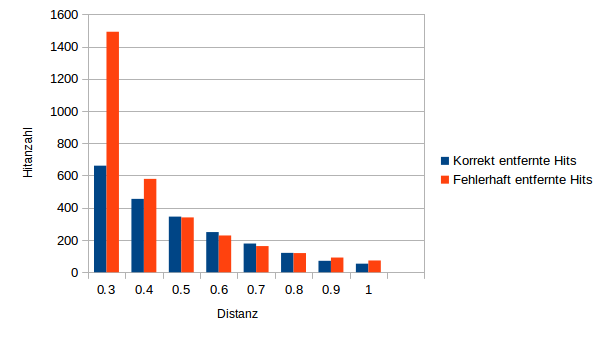
\includegraphics[width=0.9\textwidth]{Bilder/Results}
	\label{fig:results}
	\caption{Visualisierte Ergebnisse der Analysetask}
\end{center}
\end{figure}

\begin{figure}
\begin{center}
  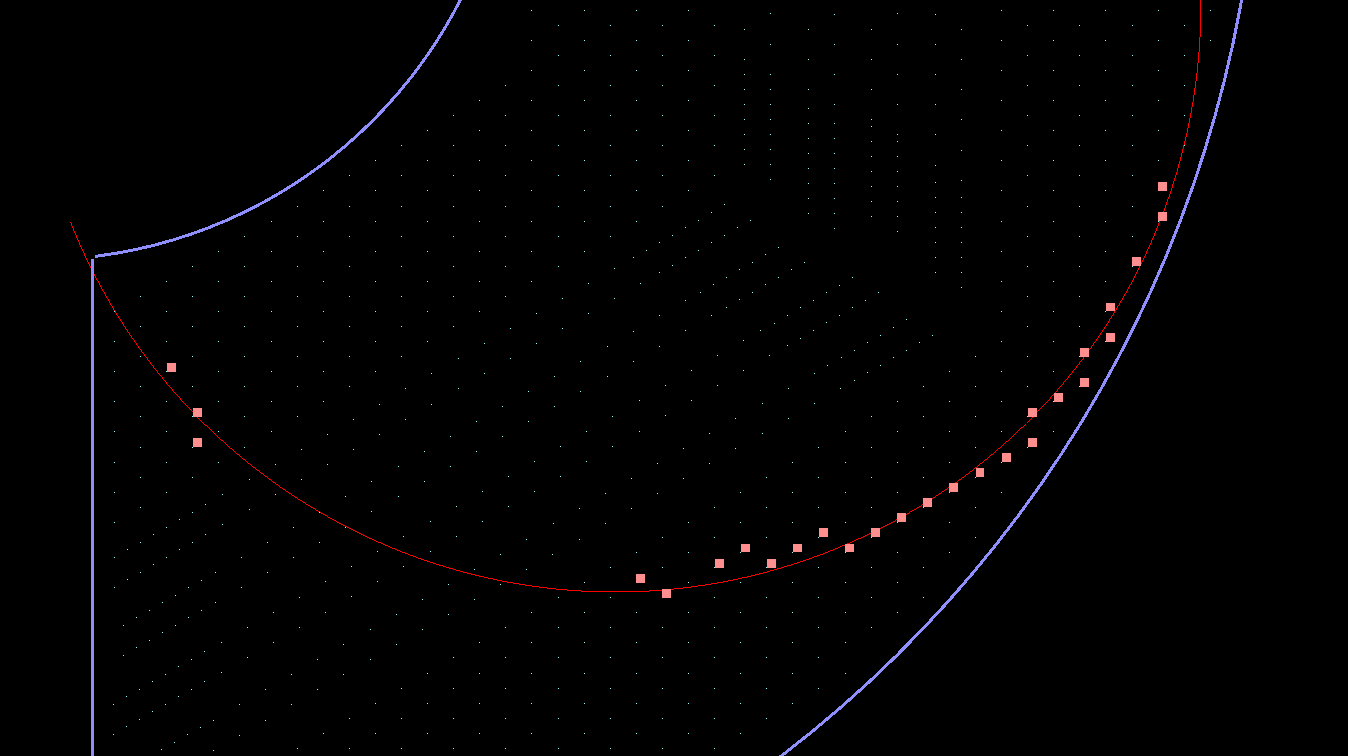
\includegraphics[width=0.9\textwidth]{Bilder/Problems}
	\label{fig:Problem}
	\caption{Visualisierung eines Events, welches beim bereinigen Probleme bereitet}
\end{center}
\end{figure}